%%Berichtvorlage für EDBV WS 2014/2015

\documentclass[deutsch]{scrartcl}
\usepackage[ngerman]{babel}
\usepackage[utf8]{inputenc}
\usepackage[T1]{fontenc}
\usepackage{algorithmic}
%%\usepackage{algorithm}
\usepackage{graphicx}
\graphicspath{ {./pictures/} }
\usepackage{amsmath,amssymb}
\usepackage{subcaption}
\captionsetup{compatibility=false}
\usepackage{multirow}
\usepackage{color}\usepackage[width=122mm,left=12mm,paperwidth=146mm,height=193mm,top=12mm,paperheight=217mm]{geometry}

\begin{document}

\title{Image Stitching} 

\subtitle{EDBV WS 2014/2015: AG\_B4} 

%%Namen und Matrikelnummern der Gruppenmitglieder hier eintragen
\author{J. Sebastian Kirchner (0926076)\\
	Hanna Huber (0925230)\\
	Patrick Wahrmann (1327120)\\
	Ernad Sehic (1227865)\\
	Nikolaus Leopold (1327344)}

%%------------------------------------------------------

\maketitle

%%------------------------------------------------------
\section{Gewählte Problemstellung}
\subsection{Ziel}
Das Ziel ist es zwei Bilder mit überlappenden Bildbereichen (also gleiche Szene mit horizontal verschobener Kamera) anhand von in beiden Bildern vorhandenen Bildmerkmalen (Interest Points) zu einem Bildmosaik zusammenzufügen, sodass die zusammengehörenden Interest Points übereinanderliegen.

\subsection{Eingabe}
Als Eingabedaten werden zwei Bilddateien im Format JPEG oder PNG, die die unten beschriebenen Voraussetzungen erfüllen, verwendet.

\subsection{Ausgabe}
Das Ergebnis ist ein Bildmosaik im selben Format wie die Eingabebilder, das aus Transformation der Einzelbilder entsteht, sodass die gemeinsamen Merkmale übereinstimmen.

\subsection{Voraussetzungen und Bedingungen}
Der Einfachheit halber werden folgende Eigenschaften der Eingabebilder vorausgesetzt:
\begin{itemize}
	\item Die Bilder sind Abbildungen der gleichen Szene, die nur horizontal versetzt sind.
	\item Es müssen überlappende Bereiche in den Bildern vorhanden sein, die kontrastreiche Interest Points aufweisen.
	\item Die Belichtungsverhältnisse müssen in beiden Bildern möglichst gleich sein (ähnliche Zeit, Ausrichtung bezüglich der Lichtquelle, gleiche Kamera!).
	\item Perspektivische Verzerrungen sollten möglichst vermieden werden, indem entfernte Motive verwendet werden und die Brennweite möglichst hoch gewählt wird.
	\item Möglichst anorganische Strukturen mit klaren Umrissen als zentrales Motiv (Bäume etc. nur am Rande).
	\item Keine beweglichen Objekte, durch die Interest Points verdeckt werden könnten.
	\item Die Bildauflösung sollte ungefähr bei 500x500 Pixel liegen (Nur grober Richtwert, Seitenverhältnisse können selbstverständlich abweichen!). Eine zu hohe Auflösung kann zu deutlich längerer Rechenzeit und möglicherweise schlechteren Ergebnissen führen. Bilder zu geringer Auflösung können unter Umständen nicht richtig zusammengesetzt werden.
\end{itemize}

\subsection{Methodik}
Der folgende Verfahrensablauf wurde implementiert:
\begin{itemize}
	\item Die Bilder werden eingelesen.
	\item Dann wird eine Bildpyramide (Difference of Gaussian, kurz DoG) für SIFT aufgebaut, mittels wiederholt ausgeführtem Gauss-Filter und Downsampling.
	\item Mithilfe der Bildpyramide werden Extrempunkte gefunden (Minima und Maxima der DoG Bilder).
	\item Unpassende Extrempunkte (geringer Kontrast, Kanten) werden entfernt, die verbleibenden Extrema sind die gesuchten Keypoints.
	\item Für Rotationsinvarianz werden die Keypoint-Umgebungsorientierungen bestimmt.
	\item In der Folge werden mittels SIFT die Keypoint-Deskriptoren erstellt.
	\item Korrespondierende Keypoints werden gefunden und zu Merkmalspaaren zusammengefasst.
	\item Mittels RANSAC (Random Sample Consensus Algorithmus) wird die homographische Transformationsmatrix ermittelt, mit der die Bilder so überandergelegt werden, dass die korrespondierenden Keypoints übereinstimmen.
\end{itemize}

Weiters wurde ein GUI implementiert.

\subsection{Evaluierungsfragen}
\begin{itemize}
	\item Werden sinnvolle Merkmale gefunden?
	\item Werden übereinstimmende Bildpaare gefunden?
	\item Werden die Bilder korrekt zusammengefügt?
	\item Hat die Auflösung der Eingabebilder einen merklichen Einfluss auf das Ergebnis?
	\item Welche Bilddaten / Szenen sind ungünstig für den Erfolg des Verfahrens?
	\item Ist das GUI intuitiv aufgebaut?
\end{itemize}


%%------------------------------------------------------

%%------------------------------------------------------
\newpage
\section{Arbeitsteilung}
Evaluierung, Datenerfassung, sowie Teile der Funktionalität und des Berichts
wurden gemeinsam erarbeitet und die Implementierungsphase war von gemeinsamem
Debugging geprägt. Speziell im Bereich der Schnittstellen wurde natürlich eng zusammengearbeitet.\\\\Die folgende Tabelle zeigt die Haupt-Aufgabenbereiche, d.h. zu den genannten Themen wurden die entsprechenden Matlab-Funktionen und Abschnitte im Bericht erstellt.
\begin{center}
  \begin{tabular}{ |l|l| }
    \hline
  Name (alphabetisch) & Tätigkeiten\\
    \hline
    \multirow{3}{*}{Hanna Huber} & Keypoint-Matching \\ & Homographische Transformation (RANSAC)\\ & Stitching (Multi-Resolution-Spline für Bildverläufe)\\ \hline
    \multirow{3}{*}{Sebastian Kirchner} & Entfernung von Keypoints die Kanten darstellen\\  & Anzeige von Keypoints und Matching\\ & Scale-Space-Erzeugung (DoGs)\\\hline
    \multirow{2}{*}{Nikolaus Leopold} & Bestimmung der Keypoint-Umgebungsorientierungen\\ & Erstellung der SIFT-Deskriptoren\\ \hline
    \multirow{1}{*}{Ernad Sehic} & Scale-Space-Erzeugung (DoGs)\\ \hline
    \multirow{3}{*}{Patrick Wahrmann} & Bestimmung der Scale-Space-Extrempunkte\\ & Entfernung von Keypoints mit geringem Kontrast\\ & GUI\\ \hline
  \end{tabular}
\end{center}

%%------------------------------------------------------

%%------------------------------------------------------
\newpage
\section{Methodik}
Ein wesentlicher Teil des Image Stitching ist die Korrespondenzanalyse. Dabei werden für den überlappenden Bereich der Bilder jene Bildpunkte in beiden Bildern gesucht, die dasselbe Objekt darstellen. Dieses Problem wird mithilfe von merkmalbasiertem Matching gelöst, das gegenüber regionenbasiertem Matching den Vorteil hat, dass homogene und daher irrelevante Bildbereiche nicht in die Berechnung mit einfließen. Der Aufwand wird dadurch erheblich reduziert. \cite{evc14} \\
Die Merkmale - Interest Points oder Keypoints - werden mittels Scale Invariant Feature Transform (kurz: SIFT) \cite{lowe04} gefunden. Dieser Algorithmus hat den Vorteil, dass das Ergebnis unabhängig von der Skalierung oder Orientierung der Interest Points im jeweiligen Bild ist \cite{evc14}.

\subsection{SIFT}
Der SIFT-Algorithmus ist in mehrere Schritte unterteilt, in denen Skalierung, Position und Orientierung der Interest Points ermittelt wird. Abschließend muss jeder Punkt eindeutig beschrieben werden, um die Korrespondenzanalyse zu ermöglichen.

\subsubsection{Bildpyramiden}
Um die Skalierungsinvarianz zu garantieren, ist eine Multiskalenanalyse der Bilder notwendig. Im Zuge dessen wird eine Bildpyramide aufgebaut, bestehend aus 4 Oktaven mit jeweils 5 Frequenzstufen. Von Oktave zu Oktave wird die Auflösung des Bildes halbiert und innerhalb der Oktaven wird iterativ gefiltert. \\
Ausgehend von dieser Bildpyramide werden nun pro Oktave 4 DoG-Bilder erstellt indem sukzessive die Differenz der gefilterten Bilder berechnet wird. 

\subsubsection{Position der Interest Points}
Interest Points stellen besonders markante, in einer lokalen Umgebung möglichst einzigartige Bildpunkte dar. Punkte, an denen sich im DoG-Bild ein lokales Minimum oder Maximum befindet, sind somit gute Kandidaten für Interest Points. Die Extrema werden in jeder Oktave der DoG-Bildpyramide gesucht. Für jedes Pixel werden dafür die umliegenden Nachbarn derselben, sowie der darüber und darunter liegenden Ebene betrachtet.\\
Um die Position des Extremums noch exakter - also im Subpixelbereich - zu bestimmen, wird danach noch eine Taylorapproximation durchgeführt.\\
Extrempunkte die wenig Kontrast aufweisen oder eine Kante darstellen, werden an dieser Stelle wieder verworfen. 



\subsubsection{Umgebungsorientierung der Keypoints}
Um Rotationsinvarianz der Keypoint-Deskriptoren zu gewährleisten, wird zusätzlich zur Keypoint-Position die Richtung maximaler Änderung, also der Gradient, der Umgebung um den Keypoint gespeichert. Die einzelnen Bestandteile des Deskriptors umfassen auch einige Orientierungen, welche nun relativ zur Grundorientierung der Umgebung definiert werden können.\\
Um die dominante Umgebungsorientierung zu beschreiben werden innerhalb eines Fensters um den Keypoint für alle Pixel die Gradienten (als Vektoren definiert durch Magnitude und Winkel) ihrer unmittelbaren 4er-Nachbarschaft bestimmt. Diese werden dann je nach ihrer Orientierung  klassifiziert (hier in 36 Teile der vollen Umdrehung von 2pi radian) und die Magnituden aller Gradienten einer Klasse (bin) aufsummiert, es wird also ein Histogramm erstellt. Dabei werden die Beiträge der Magnituden nach Gauss'scher Gewichtung um den Keypoint verteilt, sodass weiter entfernte Gradienten weniger ins Gewicht fallen. Die nach Magnitude dominante Klasse definiert nun die Orientierung der Umgebung.\cite{lowe04}

\subsubsection{Keypoint-Deskriptoren}
Um die Korrespondenzanalyse zweier Keypoints unter hunderten weiteren und unter Umständen sehr ähnlichen Keypoints zu ermöglichen, muss jeder Keypoint möglichst eindeutig beschrieben sein. Die Deskriptoren durch welche die Keypoints beschrieben werden, müssen aber auch eine gewisse Redundanz aufweisen, da sich korrespondierende Keypoints in anderen Bildern (hier in Aufnahmen derselben Szene mit anderen Einstellungen) in der Regel in Nuancen voneinander unterscheiden (Helligkeitsunterschiede, Verdeckungen, Verzerrungen, etc.). Neben einer gewissen Toleranz in der Korrespondenzanalyse (Matching) ist es daher wichtig, die Definition der für den Vergleich relevanten Grundstruktur in mehrere Teile aufzuspalten, die jeweils einen Beitrag zur Akzeptanzwahrscheinlichkeit des Keypoints liefern, sodass die Grundstruktur auch bei Abweichungen in einzelnen Teilen noch erkannt werden kann.\\
Bei SIFT werden daher die Deskriptoren durch Histogramme der Gradientenmagnituden nach 8 Orientierungsklassen (also ähnlich wie bei der Bestimmung der Umgebungsorientierung) aus 16 4*4-Fenstern um den Keypoint herum definiert. Das heißt für 16 Fenster gibt es jeweils 8 Klassen in denen Magnituden aufsummiert werden, die Definition eines SIFT-Deskriptors umfasst somit 128 Elemente.\cite{lowe04}

\subsection{Matching} 
Nun müssen Keypoints, die denselben Interest Point beschreiben, einander zugewiesen werden. Wie bei Lowe\cite{lowe04} wird dazu der Nearest-Neighbor-Ansatz gewählt.\\
Allerdings wird statt der euklidischen Distanz der Winkel zwischen den Deskriptor-Vektoren der entsprechenden Keypoints zwischen den Vektoren minimiert, der sich mithilfe des Skalarpodukt leicht berechnen lässt. \\
Um die Eindeutigkeit der Zuweisung zu garantieren, wird der kleinste Winkel mit dem zweitkleinsten verglichen\cite{lowe04}. Nur wenn deren Verhältnis unter einem Schwellwert liegt, wird die Zuweisung akzeptiert.\\
Zusätzlich wird überprüft, ob der Deskriptor mit minimalem Winkelabstand bereits einem zuvor betrachteten Deskriptor zugewiesen wurde. In diesem Fall wird dieser durch den aktuellen Deskriptor ersetzt.\\

\subsection{Homographische Transformation}
Um die beiden Bilder zu einem Bild zusammenzuführen, muss eine Homographie Matrix $H$ ermittelt werden, die die Koordinaten der Bildpunkte eines Bildes in entsprechende Koordinaten im Koordinatensystem des anderen Bildes umwandelt. Dies gilt insbesondere für Keypoint-Paare, also $X_2=H\cdot X_1$ für ein Keypoint-Paar $(X_1,X_2)$. $H$ wird mithilfe des Random Sample Consensus-Algorithmus\cite{dubrovsky09} berechnet.\\
Die Information über die Koordinaten der Keypoint-Paare wird verwendet, um ein lineares Gleichungssystem aufzustellen, dessen Lösung die Koeffizienten der Matrix $H$ liefert. Dafür werden vier Keypoint-Paare benötigt.\cite{kriegman07}\\
Der RANSAC-Algorithmus wählt diese in jedem Iterationsschritt - deren Anzahl wird zuvor festgelegt - zufällig aus und berechnet die zugehörige Matrix $H$. Daraufhin wird die Homographie auf alle zu einem Keypoint-Paar $(X_1,X_2)$ gehörigen Punkte $X_1$ angewendet. Liegt der transformierte Punkt innerhalb eines Toleranzbereichs um den Punkt $X_2$, wird er als \textit{Inlier} bezeichnet. In jedem Iterationsschritt, also für jedes $H$, wird die Anzahl der Inlier berechnet. Am Ende wird die Matrix mit den meisten Inliers als Homographie-Matrix gewählt.\\
Da eine korrekte Lösung des oben beschriebenen Gleichungssystems stark von Ursprung und Skalierung des Koordinatensystems der Bilder abhängt, werden die Koordinaten der Keypoint-Paare zuvor normalisiert. Um die endgültige Homographie-Matrix zu erhalten, wird die Matrix $H$ am Ende noch mit den entsprechenden Transformationsmatrizen multipliziert.\cite{dubrovsky09}

\subsection{Image Stitching}
Das Bildmosaik wird erstellt, indem das rechte Bild, $imB$, mithilfe der Homographie ins Koordinatensystem des linken Bildes, $imA$, transformiert wird. Um durch gerundete Daten entstehende Löcher zu vermeiden, wird dafür zunächst die Lage des transformierten Bildes im neuen Koordinatensystem ermittelt, indem die Ecken von $imB$ transformiert werden. Damit kann die Größe des Bildmosaiks berechnet werden.\\
Nun wird $imA$ entsprechend erweitert und eine Maske von derselben Größe erstellt, die die Region für das transformierte $imB$ enthält. Für diese Region werden anschließend mithilfe der inversen Homographie die entsprechenden Bildwerte berechnet. \\
Für das naive Splining wird schließlich das Bildmosaik mittels 
\begin{equation}\label{naive}
	I_{Mosaik}=(1-I_{Maske})\cdot I_{A,erweitert} + I_{Maske}\cdot I_{B,tranformiert+erweitert}
\end{equation} erstellt. \\
Für das Multiresolution Splining\cite{spline83} werden von beiden (erweiterten bzw transformierten) Bildern sowie der Maske Laplacepyramiden erstellt. Dadurch wird der Frequenzbereich in einzelne Bandbreiten von einer Oktave aufgeteilt. Nun wird auf jeder Ebene $j$ wie beim naiven Splining ein Bildmosaik zusammengesetzt:
\begin{equation}\label{mrs}
	I_{Mosaik,j}=(1-G_{Maske,j})\cdot L_{A,erweitert,j} + L_{Maske}\cdot I_{B,tranformiert+erweitert,j}
\end{equation} \\ 
Dafür werden für das linke und rechte Bild die Laplacebilder und für die Maske das Gaußbild der entsprechenden Ebene verwendet. Am Ende werden die Bilder der Mosaikpyramide schließlich zu einem Mosaik zusammengefügt.

%%------------------------------------------------------

%%------------------------------------------------------
\newpage
\section{Implementierung}
\subsection{Aufrufen der Image-Stitching-Pipeline}
\begin{itemize}
	\item gui.m 
	\item main.m 
	\item mainCMD.m
\end{itemize}
Die in Abschnitt 3 (Methodik) beschriebene Funktionalität ist in
Matlab-Funktionen gegliedert und in main.m zur kompletten
Image-Stitching-Pipeline zusammengefügt. Der Prozess wird durch mainCMD('Pfad
zum linken Bild', 'Pfad zum rechten Bild', showKeypoints, showMatches, useMRS ) gestartet, wobei die letzteren drei Parameter Boolean-Werte sind: showKeypoints bzw. showMatches zeigen vor dem fertigen Bild die gefundenen Keypoints sowie das Matching an. Ist useMRS gesetzt, wird der Multi-Resoltion-Spline-Ansatz für das Stitching verwendet, was zu weicheren Bildverläufen/-nähten führt. \\
Es ist jedoch empfohlen die grafische Oberfläche mittels Aufruf
von GUI.m zu verwenden. Alle notwendigen Schritte sind in dieser erklärt.\\
Die grafische Oberfläche ruft die Methode main auf, in der alle weiteren
Methoden der Reihe nach verwendet werden.\\\\
Für ein reibungsloses Zusammenspielen der einzelnen Komponenten sind in den Funktions-Headern die Schnittstellen definiert, also das Format der Parameter und Rückgabewerte beschrieben. Für genauere Information zu den einzelnen Funktionen sind daher diese heranzuziehen.

\subsection{Bildpyramiden}
\begin{itemize}
	\item createDog.m 
	\item createGaussPyr.m 
	\item createLog.m
\end{itemize}
Nachdem die Bilder eingelesen wurden, werden in einem ersten Schritt im Rahmen
der Methode createDoG die Bildpyramiden aufgebaut, die benötigt werden um
Interest Points zu finden. \\
In unserer Implementierung richtet sich die Implementierung bei der Erstellung der DoG-Pyramide nach Lowe \cite{lowe04}, indem wir 4 Oktaven berechnen mit jeweils 5 Frequenzstufen. Die Parameter des Gaußfilters (Sigma, Kernel) werden im Zuge der Berechnung immer neu angepasst.\\
Zu Beginn werden die Gaußbilder erstellt durch sukzessives Filtern mit Gaußfilter. Für jede Oktave wird dann die Auflösung halbiert, die Bilder der 4. Oktave haben also nur noch eine Auflösung von $\frac{1}{8} * Originalbild$.\\
Mittels dieser Pyramide werden dann die DoG-Bilder durch Differenz der aufeinanderfolgenden Gauß-Bilder in jeder Oktave ermittelt. Am Ende erhält man also pro Oktave 5 Gaußbilder und 4 DoG-Bilder.\\
Für den Multi-Resolution-Spline wird eine eigene Gaußpyramide aufgestellt, allerdings beschränkt auf 4 Levels anstatt bis zu einer Auflösung von $1x1$ Pixel Downsampling anzuwenden. Erstellt wird die Pyramide indem das Originalbild sukzessive mit einem Gaußfilter behandelt wird und die Auflösung dieses gegaußten Bildes anschließend um die Hälfte verringert wird. Der unterste Level der Pyramide ist dabei das Originalbild.\\
Die in createGaussPyr.m erstellte Gaußpyramide wird dann verwendet um die LoG-Bilder zu berechnen. Dafür wird sukzessive das Bild von einem Level höher auf der Pyramide auf die doppelte Größe skaliert und anschließend von dem Bild einen Level darunter subtrahiert, beim letzten Level ist das nicht mehr möglich, daher besteht der letzte Level der LoG-Pyramide aus dem untersten Level der Gaußpyramide. Um das Ganze etwas zu verdeutlichen:
\begin{eqnarray*}
\ LoG_0 &=& G_0 - expand(G_1) \\
\ LoG_{N-1} &=& G_{N-1} - expand(G) \\
\ LoG_N &=& G_N
\end{eqnarray*}
(expand stellt die Funktion dar, welche die Auflösung des Bildes wieder verdoppelt, in unserem Fall die Funktion imresize, als Skalierungsparameter wird dabei die Auflösung des größeren Bildes genommen, um Rundungsfehler miteinzubeziehen)

\subsection{Position der Interest Points}
\begin{itemize}
	\item findExtrema.m 
	\item removeLowContrast.m
	\item removeEdges.m
\end{itemize}
Die generierten DoG-Bilder (Difference of
Gaussians) werden daraufhin in der Funktion findExtrema auf Minima und
Maxima untersucht. Dabei wird für eine effiziente Berechnung dieser auf
einen kleinen Trick zurückgegriffen: Damit ein Pixel mit allen 26 direkten
Nachbarn schnell verglichen werden kann, wird das gesamte Bild mithilfe der
Funktion imfilter verschoben und verglichen. Die gefundenen Extrema werden
in einem weiteren Schritt in der Funktion removeLowContrast dezimiert, indem
alle potentiellen Keypoints an deren Stelle kein ausreichender Kontrast
vorliegt, verworfen werden. Um die Qualität der verwendeten Keypoints zu
verbessern, werden daraufhin in der Methode removeEdges alle Keypoints
entfernt die keine "`Ecken"' darstellen, das bedeutet Kanten werden
verworfen, da diese nicht eindeutig genug wären, um ein Matching zu
ermöglichen.\\\\
Die Methode removeEdges.m wurde implementiert, da sie Teil des Originalalgorithmus ist, wird jedoch in unserem Programm nicht verwendet, da bei Verwendung schlechtere Ergebnisse erzielt werden. 

\subsection{Keypoint-Umgebungsorientierungen}
\begin{itemize}
	\item findOrientations.m 
\end{itemize}
Im nächsten Schritt werden in der Methode findOrientations für alle Keypoints die Umgebungsorientierungen bestimmt, um Rotationsinvarianz zu gewährleisten. Wie bereits im Abschnitt Methodik beschrieben, werden dazu die Magnituden der Gradienten aller Pixel in einem 9x9-Fenster um den Keypoint nach ihren Orientierungen klassifiziert und die Magnituden aller Gradienten einer Klasse aufsummiert (es wird also ein Histogramm erstellt). Dabei wird die 4er-Nachbarschaft der Pixel betrachtet. Wichtig ist, dass die Gradienten immer in jenen Scale-Space-Stufen berechnet werden, in denen der Extrempunkt (potentieller Keypoint) gefunden wurde. Um die Orientierungen zu bestimmen, wird atan2 verwendet, da die Fallbehandlungen die bei atan notwendig sind, inkludiert sind. Die Magnituden werden in 36 Klassen (zu je 10$\,^{\circ}$) unterteilt und summiert. Dabei werden sie mit einer um den Keypoints verteilten Gauss'schen Gewichtung versehen. Die Orientierung der dominanten Klasse wird als Umgebungsorientierung des Keypoints herangezogen, wobei einfach der Median des 10$\,^{\circ}$-Intervalls gewählt wird.\cite{lowe04} 

\subsection{SIFT-Deskriptoren}
\begin{itemize}
	\item createDescriptors.m 
\end{itemize}
Nun werden, wie in Methodik beschrieben, die Keypoint-Deskriptoren erstellt. Dies geschieht in der Methode createDescriptors, wo für 16 4x4-Fenster um den Keypoint jeweils wie in findOrienations Histogramme der Gradientenmagnituden erstellt werden. Die Gauss'sche Gewichtung erfolgt dabei mit sigma von 2. Die Magnituden werden in 8 Klassen aufsummiert. Im Sinne der Rotationsinvarianz werden die Orientierungen relativ zur Keypoint-Umgebungsorientierung bestimmt. Insgesammt ergibt sich somit für einen SIFT-Deskriptor ein Vektor von 16*8 = 128 Elementen. Diese werden in Folge noch normalisiert (nach euklidischer Norm), und danach Magnituden größer als 1/5 auf diesen Wert gesetzt, um den Einfluss von Beleuchtungsunterschieden zu vermindern, (danach wird erneut normalisiert). Zu beachten ist noch, dass der Einfachheit halber Keypoints, die zu nah an den Bildrändern liegen (so dass die Fenster über den Rand hinausgehen würden), nicht berücksichtigt werden.

\subsection{Keypoint-Matching}
\begin{itemize}
	\item matchKeypoints.m
\end{itemize}
Aufgabe dieser Funktion ist es, Keypointpaare mit minimalem Winkelabstand zu finden. Dieser lässt sich leicht aus dem Skalarprodukt der beiden Vektoren ermitteln. Dafür wird über die Liste der Keypoints des ersten Bildes iteriert. Jeder Keypoint wird dabei durch den entsprechenden Zeilenindex in den Positions- und Deskriptormatrizen dargestellt. \\ 
Für jeden Deskriptor des ersten Bildes können die entsprechenden Skalarprodukte für alle Deskriptoren des zweiten Bildes mittels einer einzigen Vektor-Matrix-Multiplikation berechnet werden. Der Vektor der zugehörigen Winkel wird daraufhin sortiert, der kleinste gewählt und der entsprechende Deskriptor des zweiten Bildes identifiziert und dessen Index abgespeichert. Die entsprechende Variable $matchInd$ hat die Form $matchInd( Index_{Keypoint in Bild1} ) = Index_{Keypoint in Bild 2}$. Auch der Winkelabstand wird abgespeichert. \\
Als Schwellwert für den Vergleich zwischen kleinstem und zweitkleinstem Winkelabstand wird der Wert 0.6 von Weyand\cite{pandemo} übernommen. \\
Falls $Index_{Keypoint in Bild 2}$ bereits in $matchInd$ abgespeichert wurde, werden die Winkelabstände verglichen. Ist der aktuelle Wert kleiner, wird $Index_{Keypoint in Bild 2}$ an früherer Stelle durch 0 ersetzt. \\
Am Ende werden die Positionen der zugeordneten Paare\\$matchInd(Index_{Keypoint in Bild1} \neq 0)$  zurückgegeben.

\subsection{Homographische Transformation}
\begin{itemize}
	\item findHomography.m 
	\item fitSample.m 
	\item normalizeSample.m
	\item normalizationMatrix.m
\end{itemize}
In findHomography.m ist der RANSAC-Algorithmus implementiert. Der von Weyand\cite{pandemo} empfohlenen Anzahl an Iterationen, $10 \cdot 2^{AnzahlMatches}$, wurde eine obere Schranke von $10^4$ Iterationen hinzugefügt.\\\\
Das mittels $datasample$ ausgewählte Sample von Matches wird mittels normalizeSample.m normalisiert. normalizeSample.m verwendet dabei die Tranformationsmatrizen, die mithilfe von normalizationMatrix.m berechnet werden. Anschließend berechnet fitSample.m die entsprechende Homographie Matrix $H$. \\\\
Nun wird $H$ in findHomographie auf alle Keypointpaare angewendet und die Inliers werden gezählt.Dabei wird die euklidische Distanz zwischen dem transformierten Punkt und dem zweiten Punkt des Keypointpaares berechnet. Als Schwellwert wird hierbei der Wert 0.02 verwendet. Gegenbenenfalls wird die bis zu diesem Punkt beste Matrix $Hbest$ durch die aktuelle ersetzt. Am Ende wird $Hbest$ zurückgegeben.

\subsection{Stitching}
\begin{itemize}
	\item stitchImages.m 
	\item multiResSpline.m 
	\item replicateEdge.m
\end{itemize}
Zunächst werden die Koordinaten der Eckpunkte des rechten Bildes mithilfe der Homographie-Matrix $HBtoA$ ins Koordinatensystem des linken Bildes transformiert. Dadurch kann die Lage des Bildes und somit die Größe des Bildmosaiks bestimmt werden. Liegt das rechte Bild an manchen Stellen oberhalb des linken Bildes, ist zusätzlich eine Verschiebung in den positiven Koordinatenbereich nötig. \\\\
Als nächstes werden die Bildwerte des linken Bildes unter Verwendung der Lageinformation bzw. Verschiebung in das noch leere Bildmosaik eingetragen. \\
Eine weitere Matrix derselben Größe wird erstellt, die die Werte des zweiten Bildes an der entsprechenden Stelle enthalten soll. Mithilfe der (verschobenen) transformierten Eckpunkte wird eine Maske erstellt, die angibt, welche Punkte im Bildmosaik Bildwerte des rechten Bildes enthalten sollen. Um die entsprechenden Werte zu berechnen, wird diese Maske zurückverschoben und die ursprünglichen Koordinaten werden mittels $HAtoB$ ermittelt. Nun können die Bildwerte in die zweite leere Matrix eingetragen werden. \\\\
Falls das endgültige Bildmosaik mittels Multiresolution-Spline zusammengefügt werden soll, wird das rechte Bild innerhalb des Mosaiks ein wenig erweitert, indem die Werte an der Kante in die entsprechende Richtung repliziert werden. Dadurch werden die Kanten, die an der Grenze zwischen Bildwerten und Nulleinträgen der Matrix entstehen, verschoben. Das das Splining mit Laplacepyramiden arbeitet, würden diese Kanten andernfalls entlang der Naht unerwünschte Effekte hervorrufen. Der Parameter $width$ bestimmt das Ausmaß der Replikation und wird auf 10 (d.h. zehn Zeilen bzw. Spalten) gesetzt. Größere Werte führen zu unerwünschten Unschärfeeffekten. Sollte der Abstand zwischen Naht und Bildrand geringer sein, wird dies berücksichtigt. \\
 Da die Maske unverändert bleibt, wird das Bild im endgültigen Mosaik nicht erweitert. \\
Dieses wird in multeResSpline.m zusammengesetzt. Dafür werden Laplacepyramiden für beide Bilder erstellt. Zusätzlich wird eine Gaußpyramide für die Maske erstellt, was die Übergänge weicher macht. Nach \eqref{mrs} wird das endgültige Mosaik auf jeder Ebene separat zusammengefügt. Am Ende wird die Pyramide wiederzusammengsetzt und das Bildmosaik zurückgegeben. \\\\
Ohne Multiresolution-Spline wird das Mosaik bereits nach dem Einfügen des transformierten Bildes in das zweite leere Mosaik mittels \eqref{naive} zusammengefügt.

\subsection{Anzeige Keypoints bzw. Matching}
\begin{itemize}
	\item showKeypoints.m
	\item showMatches.m
\end{itemize}
Die Funktionen showKeypoints.m und showMatches.m können verwendet werden um die Position der Keypoints im Bild anzuzeigen. Bei showKeypoints können zusätzlich Orientierungen als Eingabeparameter übergeben werden um diese ebenfalls anzuzeigen. Sollen keine Orientierungen angezeigt werden, so kann man diesen Input einfach auslassen.\\\\
Die Funktion showMatches kann benutzt werden um anzuzeigen welche Keypoints in den beiden Input-Bildern zugeordnet wurden, dafür müssen die Parameter für die Keypoints allerdings richtig geordnet und gleich lang sein, es empfiehlt sich der Aufruf also immer nur nach der Funktion matchKeypoints. Hier kann man auch sehr leicht sehen ob die Keypoints korrekt zugeordnet wurden oder nicht.
%%------------------------------------------------------

%%------------------------------------------------------
\newpage
\section{Evaluierung}

\subsection{Datensatz}

\begin{figure}[p]
\begin{center}
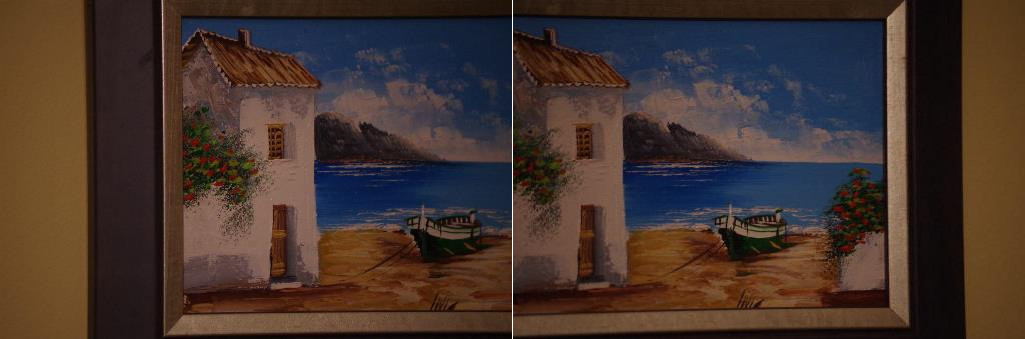
\includegraphics[width=1.0\textwidth]{strand.jpg}
\caption{strand: links und rechts}
\label{fig:strand}
\end{center}
\end{figure}

\begin{figure}[p]
\begin{center}
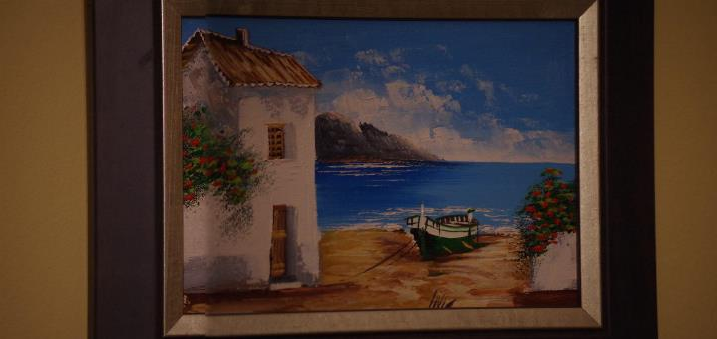
\includegraphics[width=1.0\textwidth]{strandS.png}
\caption{strand: stitched}
\label{fig:strandS}
\end{center}
\end{figure}

\begin{figure}[p]
\begin{center}
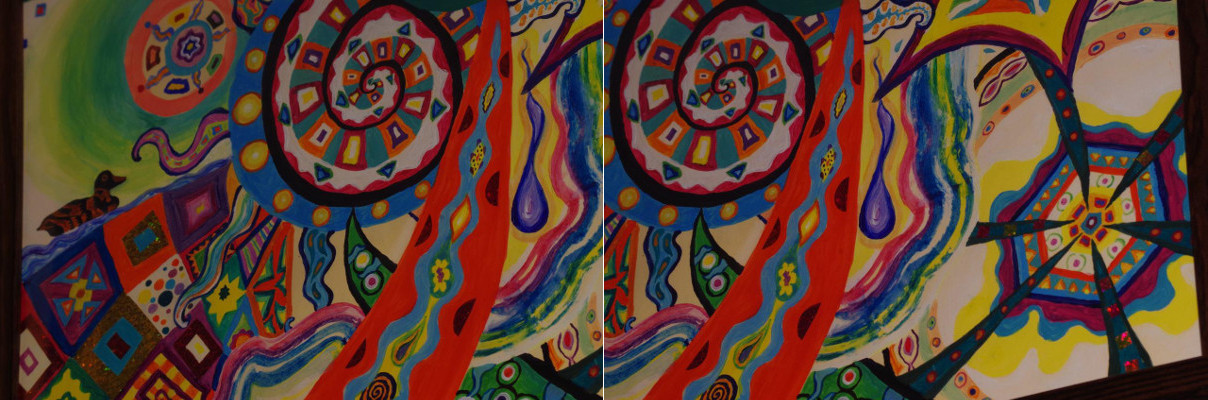
\includegraphics[width=1.0\textwidth]{bunt.jpg}
\caption{bunt: links und rechts}
\label{fig:bunt}
\end{center}
\end{figure}

\begin{figure}[p]
\begin{center}
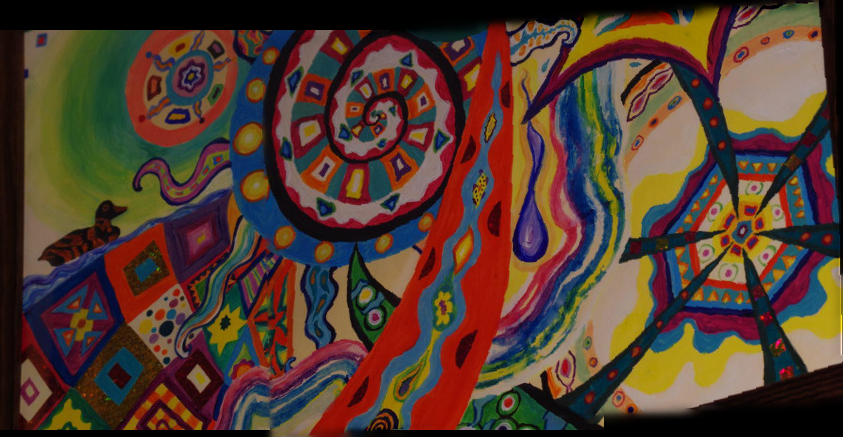
\includegraphics[width=1.0\textwidth]{buntS.png}
\caption{bunt: stitched}
\label{fig:buntS}
\end{center}
\end{figure}

\begin{figure}[p]
\begin{center}
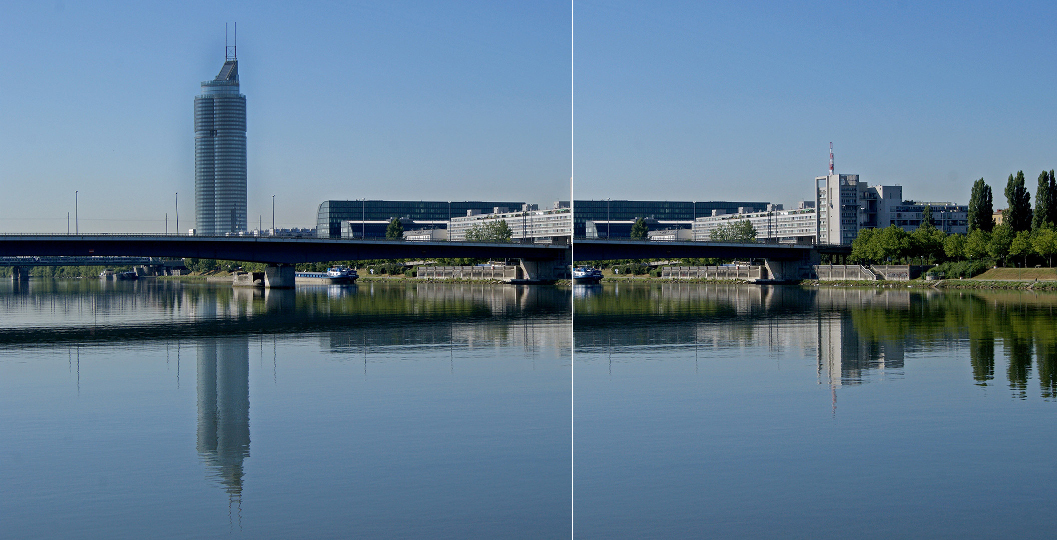
\includegraphics[width=1.0\textwidth]{tower.jpg}
\caption{tower: links und rechts}
\label{fig:tower}
\end{center}
\end{figure}

\begin{figure}[p]
\begin{center}
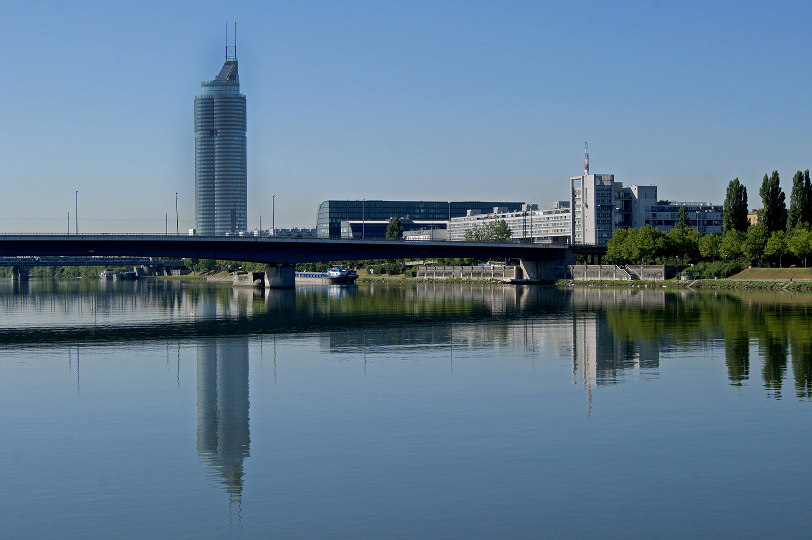
\includegraphics[width=1.0\textwidth]{towerS.png}
\caption{tower: stitched}
\label{fig:towerS}
\end{center}
\end{figure}

\begin{figure}[p]
\begin{center}
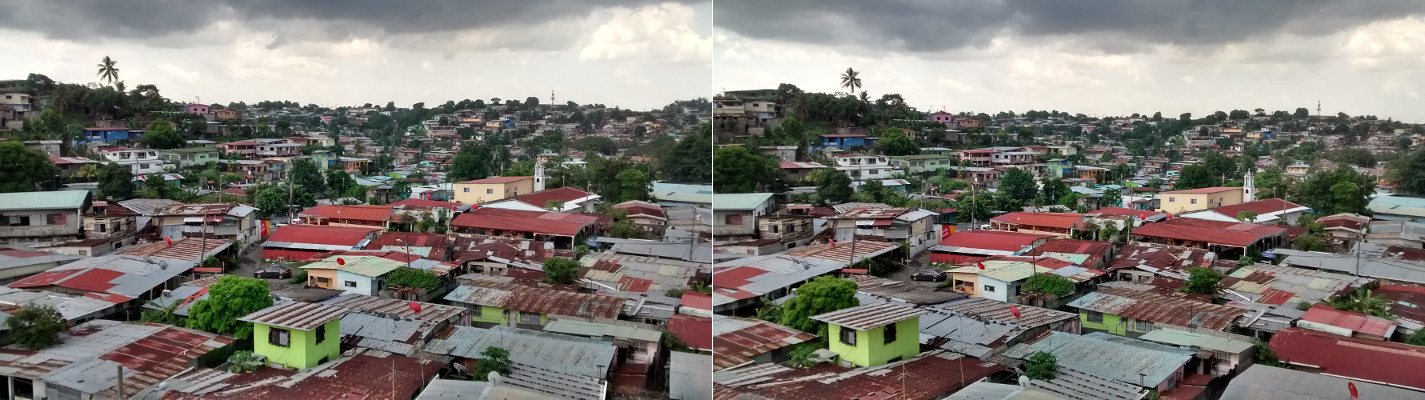
\includegraphics[width=1.0\textwidth]{sanmiguelito.jpg}
\caption{sanmiguelito: links und rechts}
\label{fig:sanmiguelito}
\end{center}
\end{figure}

\begin{figure}[p]
\begin{center}
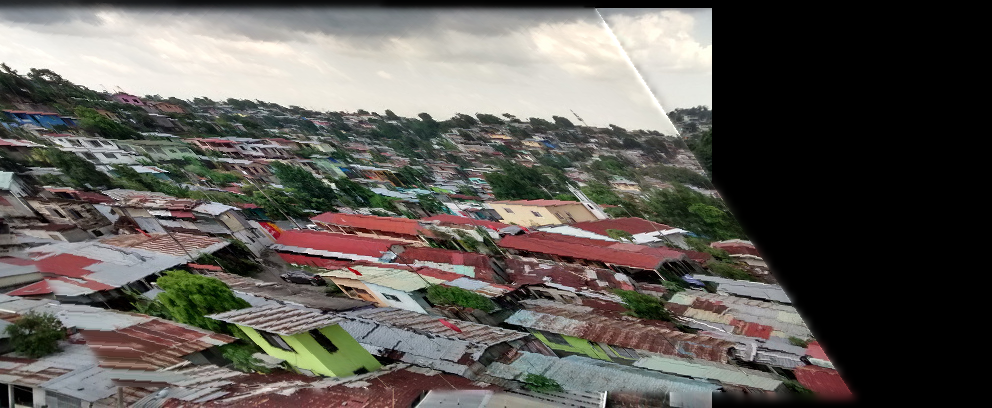
\includegraphics[width=1.0\textwidth]{sanmiguelitoS.png}
\caption{sanmiguelito: stitched}
\label{fig:sanmiguelitoS}
\end{center}
\end{figure}

\begin{figure}[p]
\begin{center}
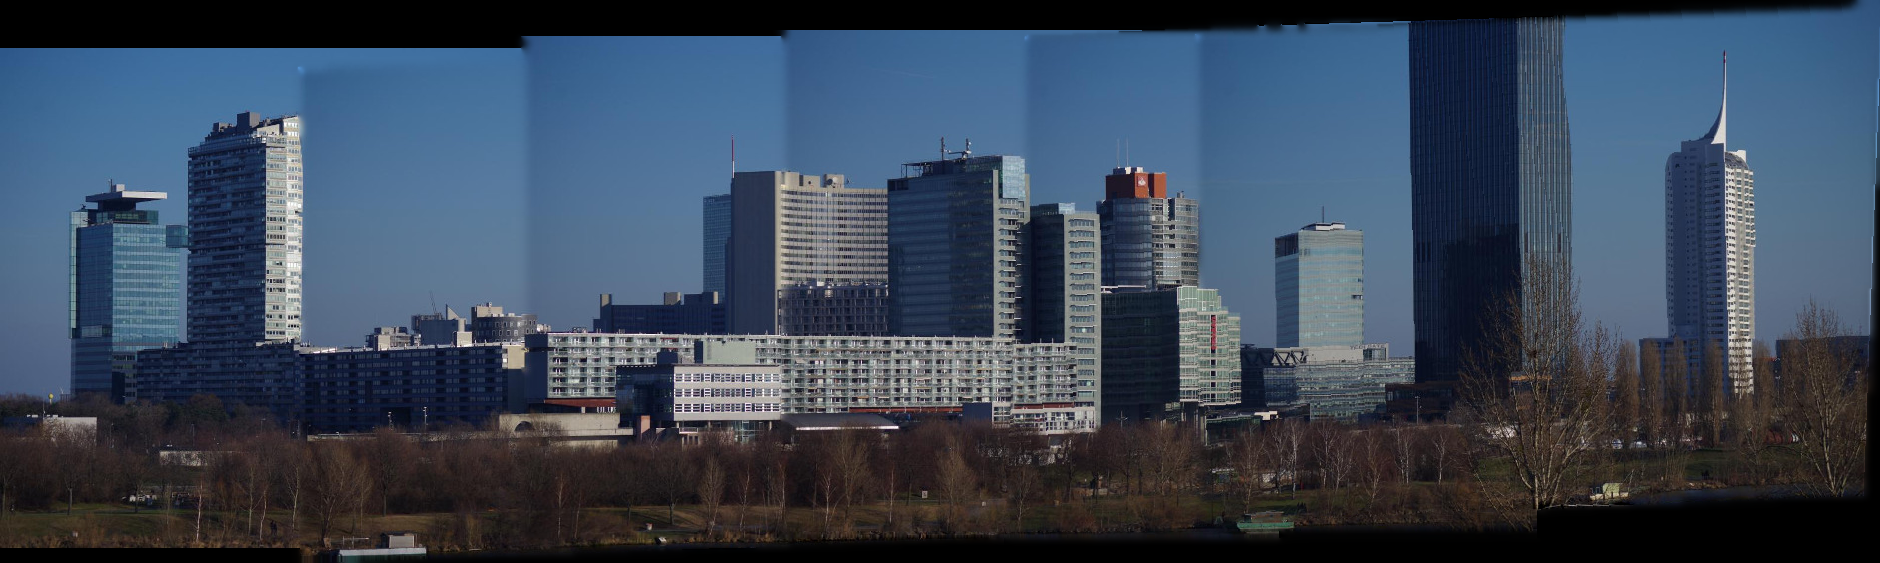
\includegraphics[width=1.0\textwidth]{skylineS.png}
\caption{skyline: stitched}
\label{fig:skylineS}
\end{center}
\end{figure}

\begin{figure}[p]
\begin{center}
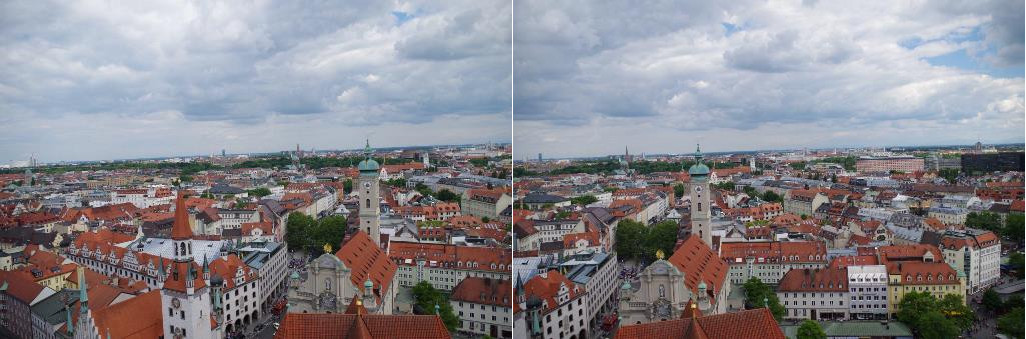
\includegraphics[width=1.0\textwidth]{munich.jpg}
\caption{munich: links und rechts}
\label{fig:munich}
\end{center}
\end{figure}

\begin{figure}[p]
\begin{center}
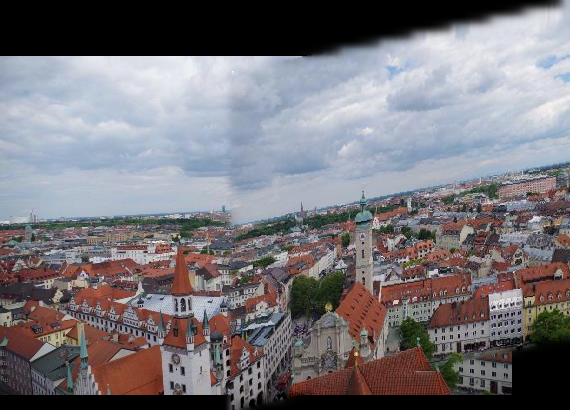
\includegraphics[width=1.0\textwidth]{munichS.png}
\caption{munich: stitched}
\label{fig:munichS}
\end{center}
\end{figure}

\begin{figure}[p]
\begin{center}
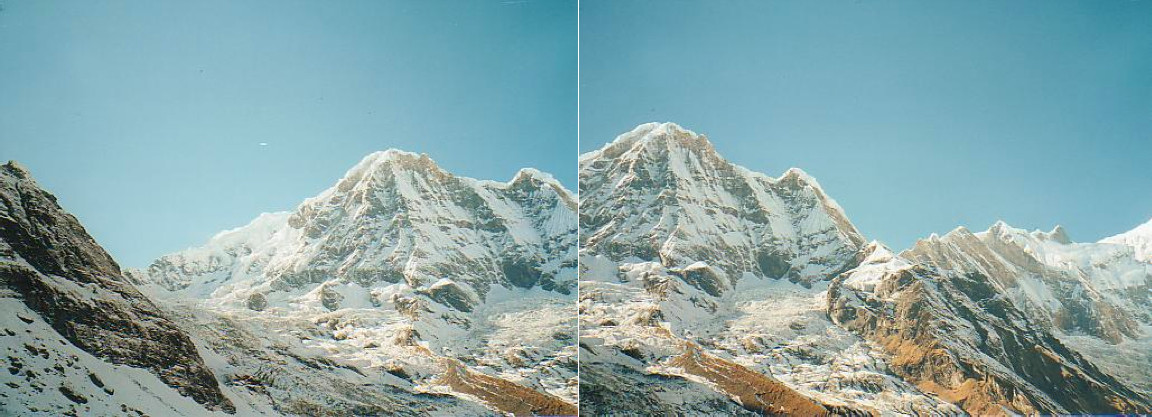
\includegraphics[width=1.0\textwidth]{demo.jpg}
\caption{demo: links und rechts}
\label{fig:demo}
\end{center}
\end{figure}

\begin{figure}[p]
\begin{center}
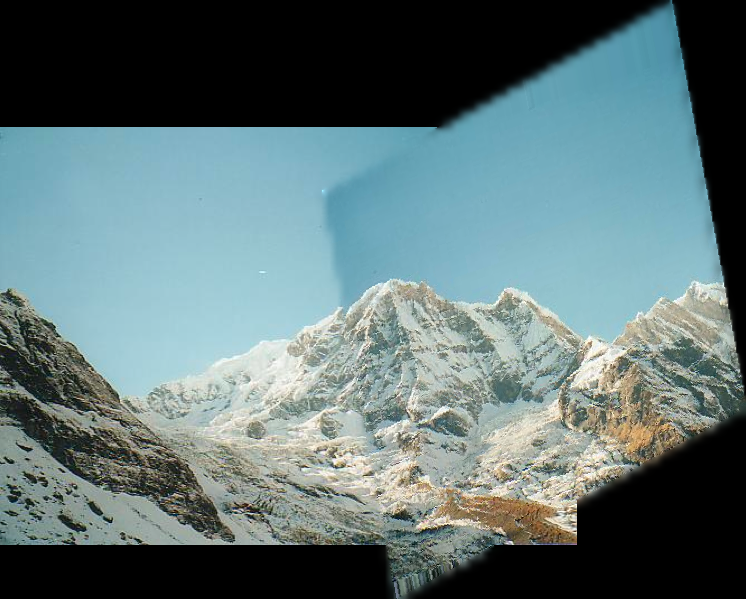
\includegraphics[width=1.0\textwidth]{demoS.png}
\caption{demo: stitched}
\label{fig:demoS}
\end{center}
\end{figure}

\begin{figure}[p]
\begin{center}
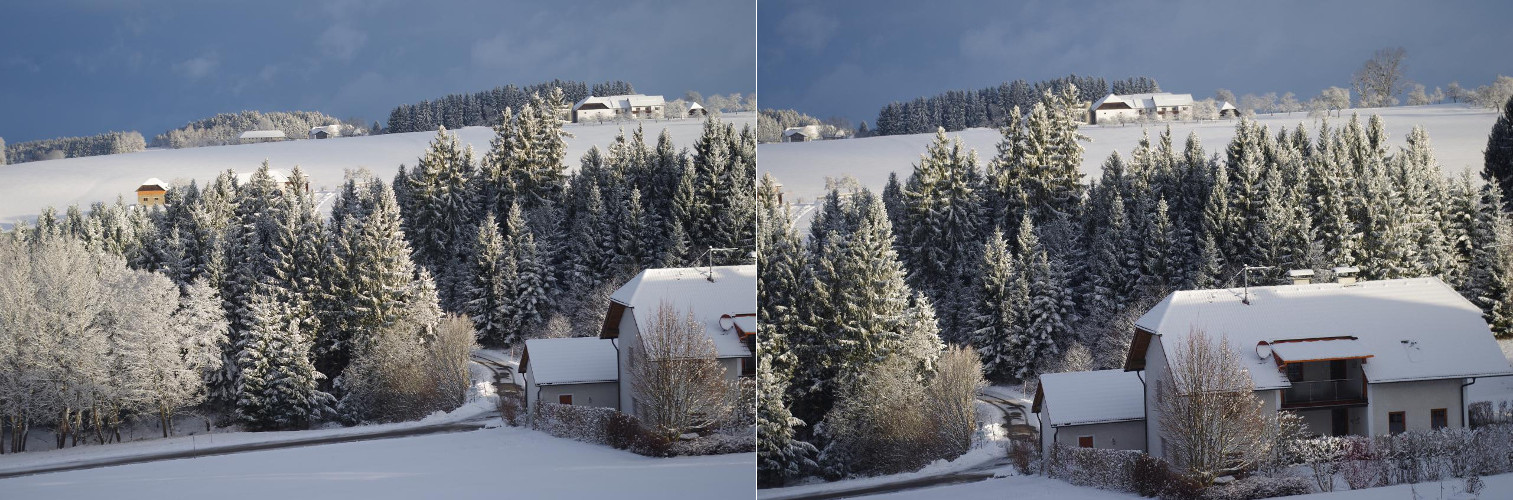
\includegraphics[width=1.0\textwidth]{winter.jpg}
\caption{winter: links und rechts}
\label{fig:winter}
\end{center}
\end{figure}

\begin{figure}[p]
\begin{center}
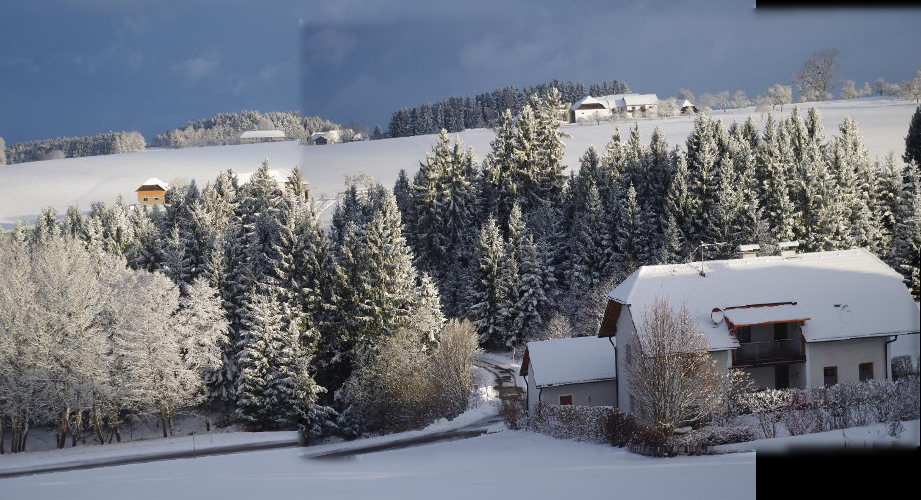
\includegraphics[width=1.0\textwidth]{winterS.png}
\caption{winter: stitched}
\label{fig:winterS}
\end{center}
\end{figure}

\begin{itemize}
	\item strand.jpg\\
		Quelle: Patrick Wahrman\\
		Aufnahmegerät: Spiegelreflexkamera Pentax K30 \\
		Einstellungen für beide Bilder: \\
		Brennweite: 200mm \\
		Belichtungszeit: 2s \\
		Blendenzahl: 3.5

	\item winter.jpg\\
		Quelle: Patrick Wahrman\\
		Aufnahmegerät: Spiegelreflexkamera Pentax K30 \\
		Einstellungen für beide Bilder: \\
		Brennweite: 120mm \\
		Belichtungszeit: 1/100s \\
		Blendenzahl: 3.5.

	\item bunt.jpg\\
		Quelle: Patrick Wahrman\\
		Aufnahmegerät: Spiegelreflexkamera Pentax K30 \\
		Einstellungen für beide Bilder: \\
		Brennweite: 200mm \\
		Belichtungszeit: 2s\\
		Blendenzahl: 3.5.

	\item tower.jpg\\
		Quelle: Ernad Sehic\\
		Aufnahmegerät: Spiegelreflexkamera Sony \\
		Einstellungen für beide Geräte: \\
		Brennweite: 35mm \\
		Belichtungszeit: 1/250s \\
		Blendenzahl: 13.

	\item sanmiguelito.jpg\\
		Quelle: Nikolaus Leopold \\
		Aufnahmegerät: gewöhnliche Digitalkamera Canon\\
		Standardeinstellungen für beide Bilder

	\item demo.jpg\\
		Quelle: \cite{pandemo}

	\item munich.jpg\\
		Quelle: Patrick Wahrman\\
		Aufnahmegerät: Spiegelreflexkamera Pentax K30 \\
		Einstellungen für beide Geräte: \\
		Brennweite: 120mm \\
		Belichtungszeit: 1/40s \\
		Blendenzahl: 3.5.

	\item skyline.jpg\\
		Quelle: Patrick Wahrnamm\\
		Aufnahmegerät: Spiegelreflexkamera Pentax K30 \\
		Einstellungen für beide Geräte: \\
		Brennweite: 120mm \\
		Belichtungszeit: 1/100s\\
		Blendenzahl: 3.5.
\end{itemize}

\subsection{Diskussion der Evaluierungsfragen}

\begin{itemize}
	\item Werden sinnvolle Merkmale gefunden? 
		Ja. Die gefundenen Keypoints befinden sich an geeigneten Stellen im Bild und zeigen die korrekte Umgebungsorientierung.
	\item Werden übereinstimmende Bildpaare gefunden? 
		Obwohl vereinzelt auch nicht zusammenpassende Keypointpaare detektiert werden, wird die Zuordnung generell erfolgreich ausgeführt.
	\item Werden die Bilder korrekt zusammengefügt? 
		Abhängig von der perspektivischen Verzerrung der Bilder funktioniert das Image Stitching generell gut bis sehr gut (siehe Abbildungen \ref{fig:strand} und \ref{fig:strandS} bzw Abbildung \ref{fig:skylineS}). In Bildbereichen, in denen keine Matches gefunden werden, können die Übergänge jedoch teilweise fehlerhaft sein (siehe Abbildungen \ref{fig:winter} und \ref{fig:winterS} bzw Abbildungen \ref{fig:demo} und \ref{fig:demoS}).
	\item Hat die Auflösung der Eingabebilder einen merklichen Einfluss auf das Ergebnis? 
		Innerhalb des empfohlenen Rahmens gibt es keine ersichtlichen Unterschiede. Bei einer zu hohen Auflösung ist der Rechenaufwand zu groß und ein korrektes Ergebnis kann nicht garantiert werden. 
	\item Welche Bilddaten / Szenen sind ungünstig für den Erfolg des Verfahrens? 
		Das rechte Bild darf keine Bereiche darstellen, die links vom linken Bild liegen (siehe Abbildungen \ref{fig:sanmiguelito} und \ref{fig:sanmiguelitoS}). Perspektivische Verzerrungen führen ebenfalls zu Fehlern, Rotationen dürfen also lediglich in der xy-Ebene stattfinden (siehe Abbildungen \ref{fig:munich} und \ref{fig:munichS}). Dazu sind unterschiedliche oder schlechte , wie z.B. am Abend vorherrschende, Lichtverhältnisse problematisch.
	\item Ist das GUI intuitiv aufgebaut?
		Das GUI ist simpel gestaltet und selbsterklärend. Die Mouseover-Funktion liefert zusätzliche Informationen.
\end{itemize}
%%------------------------------------------------------

%%------------------------------------------------------
\newpage
\section{Schlusswort}
Da der SIFT-Algorithmus eine hohe Komplexität aufweist, haben wir uns bereits zu Beginn für eine Einschränkung der möglichen Inputbilder entschieden. Es war unser Anspruch, die Ergebnisse des Originalalgorithmus lediglich für diese eingeschränkte Auswahl und auch nicht in vergleichbarer Qualität zu reproduzieren. \\
Im Zuge unserer Arbeit wurden diese Vorgaben geringfügig erweitert, jedoch im Allgemeinen eingehalten.\\\\
Für Bilder, die die vorgegebenen Voraussetzungen erfüllen, werden beim Image Stitching gute bis sehr gute Ergebnisse erzielt. Sobald die Inputdaten allerdings von den Vorgaben abweichen, sind die Resultate sehr fehlerhaft. Man könnte das Programm deshalb noch dahingehend verbessern, dass es weniger anfällig für Abweichungen ist und auch momentan ausgeschlossene Daten wie perspektivisch verzerrte Bilder erfolgreich gestitcht werden.\\\\
Uns war bewusst, dass es sich bei SIFT um state-of-the-art Technologie handelt, und dass wir kaum eine vollständige Implementierung des von Lowe\cite{lowe04} beschriebenen Algorithmus erzielen würden. Bei der Wahl des Themas waren wir uns der Herausforderung bewusst. Insgesamt sind wir daher zufrieden mit dem Ergebnis!\\
%%------------------------------------------------------

%%------------------------------------------------------
\newpage
\bibliographystyle{plain}
\bibliography{edbv_lit}
%%Bei verwendung von Latex schreibt ihr eure Referenzen in ein eigenes bib-File (siehe hier edbv_lit.bib). Jene Referenzen, die ihr im Bericht mittels \cite zitiert, werden automatisch in die Referenzliste übernommen. Weitere Information zum Einbinden von BibTex gibt es hier: http://www.bibtex.org/Using/de/
%%------------------------------------------------------

\end{document}
